\documentclass{abntpuc}

\usepackage[pdftex]{graphicx}

\usepackage{fancyhdr}

\begin{document}

% --- Campos que formarao: capa, folha de rosto, folha de aprovacao  ---

\curso{Bacharelado em Sistemas de Informação}

\autor{Alexandre Gonzaga Mendes}

\titulo{DEFINIR O NOME} % Caixa alta

\subtitulo{Subtítulo do Trabalho} % Caixa baixa

\cidade{Belo Horizonte}

\ano{2013}

\trabalho{Monografia} % Tipo de trabalho: Monografia, Dissertacao, Tese...

\grau{Bacharel em Sistemas de Informação} % Grau do trabalho: Bacharel em..., Mestre em..., Doutor em...

\orientador{João Caram Adriano}

\avaliadorA{Nome do Avaliador 1}

\avaliadorB{Nome do Avaliador 2}

\datacompleta{DD de MM de 2013} % Dia, mes e ano

% --- CAPA ---

\capa

% --- FOLHA DE ROSTO ---

\folharosto

% --- FOLHA DE APROVACAO ---

\folhaaprovacao

% --- DEDICATORIA (elemento opcional) ---

\dedicatoria
{
\textit{Dedicatória: Página onde o autor presta homenagem a uma ou mais pessoas.
O layout desta página fica a critério do autor, mas o tipo e tamanho de letras são definidos pela ABNT.}
}

% --- AGRADECIMENTOS (elemento opcional) ---

\agradecimentos
{
Agradecimentos a pessoas que contribuíram para o desenvolvimento do trabalho.
Agradecimentos a pessoas que contribuíram para o desenvolvimento do trabalho.
}

% --- EPIGRAFE (elemento opcional) ---

\epigrafe
{
\textit{Epígrafe: Pensamentos retirados de um livro, uma música, um poema, normalmente relacionados ao tema do trabalho.
Deve ser elaborada conforme norma NBR 10520/2002. Apresentação de citações em documentos.
Se desejar, a epígrafe pode ser grafada em itálico.
Ao final do trabalho deve-se fazer a referência completa da publicação de onde a epígrafe foi retirada.}
}

% --- RESUMO ---

\resumo
{
Apresentação concisa dos pontos relevantes do texto. Deve ressaltar o objetivo, o método, resultados e conclusões do trabalho. Deve-se utilizar o verbo na voz ativa ou terceira pessoa do singular. O resumo não deve conter citações ou indicações bibliográficas.
} % Resumo
{
Ao final do resumo deve-se elaborar palavras-chave representativas do conteúdo do trabalho, separadas entre si por um ponto.
} % Palavras-chave

% --- ABSTRACT ---

\abstract
{
Versão do resumo em idioma de divulgação internacional. Deve ser a tradução literal do resumo em português e apresentar palavras- chave no mesmo idioma, logo abaixo do texto, separadas entre si por um ponto.
} % Abstract
{
O resumo em língua estrangeira também deve conter palavras-chave representativas do conteúdo do trabalho, separadas entre si por um ponto.
} % Keywords

% --- LISTA DE FIGURAS, LISTA DE TABELAS, SUMARIO ---

\listafiguras
\listatabelas
\listasiglas {
\sigla{S1}{Sigla 1}
\sigla{S2}{Sigla 2}
\sigla{S3}{Sigla 3}
}


% --- TEXTO ---

\sumario
\capitulo{INTRODUÇÃO}

\secao{Contextualização}

Instituições de ensino universitarias se deparam todo início de semestre letivo com o problema de alocação de salas, este problema pode ser definido como \textit{Classroom Assignment} que é uma instancia do \textit{course timetabling}, problemas desta instancia são prolemas de otimização combinatoria. Problemas de otimização combinatoria tem a complexidade NP-difícil, para a resolução de problemas desta complexidade em um tempo razoavel são propostas algumas tecnicas denominadas meta-heuristicas. Esta técnicas amenizam a dificildade da resolução destes problemas para encontrar uma solução em um tempo habil, uma vez que, a resolução destes problemas de forma manual é de grande dificuldade em alguns casos pode demandar semanas de trabalho da pessoa responsável.\par


Em suma o trabalho consiste na distruições das disciplinas pertecentes aos cursos de graduação e pós-graduação apresentados po alguns  colegiados da Universidade Federal de Minas Gerais (UFMG) , em salas disponibilizadas pelo predio da Faculdade de Filosofia e Ciências Humandas (FAFICH). Para a distribuição destas disciplinas nas salas, foi criado um sistema que utiliza conceitos de algorítimo genético para resolver o problema PAS. Esta demanda de alocação acontece todo início de semestre e é executada assim que todos os colegiados tenham enviados suas solicitações necessidas para aquele semestre.\par

Uma vez que os termos da biologia utilizados foram lincados com o problema, o sistema gera uma alocação com grandes chances de atender as necessidades da instituição. \par

\secao{Objetivos}

O tratamento do problema de alocação de salas em instituições de ensino carece de bons trabalhos na literatura. Apesar de se encontrar ferramentas disponíveis, poucas tratam de maneira eficiente as restrições reais existentes nas instiruições. Com este trabalho objetiva-se:

\subsecao{Objetivos Gerais}

O objetivo deste trabalho é utilizar os conceitos de algoritimo genético para a resolução dos problemas denominados PAS através do desenvolvimento de um sistema que atenda todas as necesssidades da instiruição e facilite o gerenciamento das informações da instituição como salas, disciplinas e demais informações.

\subsecao{Objetivos Específicos}

	- Desenvolvimento do sistema.\par

	- Implementação de um algoritmo que proporcione uma solução de qualidade.

	- Otimizar o tempo do gestor.\par

	- Eficiência na geração dos relatórios.\par

\secao{Justificativa}

A solução de problemas de PAS através de meta-heurísticas se trata de uma área ainda não consolidada, por mais que existam trabalhos relacionados ao tema espera-se que as conclusões realizadas neste trabalho agreguem valor algum falor para os trabalhos futuros.

\secao{Organização do Trabalho}

Este trabalho está definido da seguinte forma, foi dividido em seis capítulos, sendo este capítulo 1 e mais cinco outros.\par

O capítulo 2 apresenta o referencial teórico do trabalho, descrevendo os conceitos utilizados para o desenvolvimento do projeto proposto: conceitos de TimeTable e Heurísticas.\par

No capítulo 3 é apresentada a metodologia do sistema e as tecnologias adotadas para desenvolvimento da solução.\par

No capítulo 4 iremos descrever e citar detalhadamente as características e propostas de desenvolvimento do sistema desenvolvido, proposto para este trabalho.\par

A conclusão deste trabalho e considerações finais são mostrados nos capítulos 5 e 6.\par

\capitulo{REVISÃO LITERARIA}

\secao{Descricão do problema}
Escrever sobre os objetivos e as justificativas

\secao{Complexidade do problema}
Este trabalho está definido da sequinte forma. Capitulo 1 Capitulo 2 Capitulo 3 Capitulo 4 

\secao{Métodos}

%
\capitulo{METODOLOGIA}

\iniciocapitulo
A resolução deste trabalho está dividida nas seguintes partes instalação do ambiente, análise e algorítimo.\par

A implementação do sistema se deve primeiramente a configuração do ambiente para o início do desenvolvimento os seguintes passos devem ser tomados para que o ambiente seja reproduzido novamente. Primeiramente deve se instalar o SGBD PostgreSQL, logo em seguida deve se instalar o JAVA 7 em sua maquina, para validar a instalação deve-se executar o seguinte comando "java -version && javac -version" a mensagem descrita na figura XX deve ser mostrada.

\begin{figure}[!htb]
\caption[Versão Java]{Versão Java}
\label{fig:figura2}
\centering
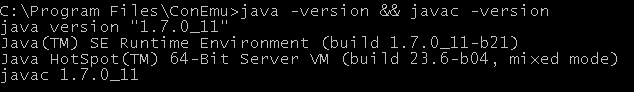
\includegraphics[scale=0.8]{imagens/mensagemJava.png}
\\ \textbf{\footnotesize Fonte: Autor}
\end{figure}


Após a instalação do java deve-se instalar o framework Play! seguindo os passos encontrados no site \cite{play} para validar a instalação do Play! deve se executar o comando "play version" e o \textit{prompt} de comando deve retornar a mensagem conforme mostra a figura figura XX.

\begin{figure}[!htb]
\caption[Versão Framework]{Versão Framework}
\label{fig:figura2}
\centering
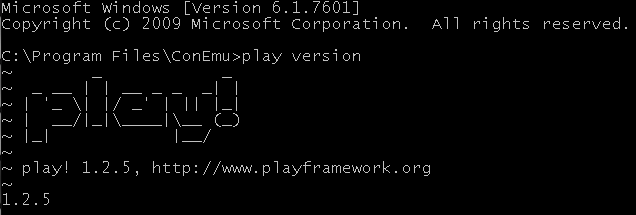
\includegraphics[scale=0.8]{imagens/mensagemPlay.png}
\\ \textbf{\footnotesize Fonte: Autor}
\end{figure}

Uma vez que o ambiente já está configurado devemos inciar um projeto no framework instalado através do comando "play new nomeDoProjeto", a partir dai é possível escolher IDE que será utilizada.

Foi criado um \textit{script} para criação do banco de dados e população inicial das informações como, prédios, salas, turnos, horários, e disciplinas com informações que são necessárias em todo inicio de semestre na instituição de ensino escolhida.

PQ do algoritimo genetico
segundo renand dupas a escolha de algoritimoes geneticos se dá através de uma comparação com outras técnicas e através disso de uma evidenciação das vantagens de sua utilização , logo o algoritimo genetico foi escolhido para este trabalho.

População inicial = --UMA NOVA ABORDAGEM PARA AUMENTAR A DIVERSIDADE.pdf

modelo matematico ----APLICAÇÃO DE MODELO MATEMÁTICO, ABORDAGEM HEURÍSTICA E MÉTODO MISTO NA OTIMIZAÇÃO DA PROGRAMAÇÃO DE HORÁRIO DOS PROFESSORESTURMAS.pdf

restrições do problema e modelo matematico http://www.dcc.ufla.br/infocomp/artigos/v4.3/art08.pdf

Foi realizada uma análise dos requisistos atravez de entrevista com o steakholder, após as entrevistas a modelagem de dados foi realizada de acordo com a demanda do projeto, para o desenvolvimento destes diagramas foi utilizadas a UML (Universal Modeling Language). Os seguintes diagramas foram desenhados, diagrama de caso de uso, diagrama de classe e diagrama de entidade relacionamento. Foram escolhidos os seguintes diagramas para que o sistema tenha uma documentação minima tendo em vista que o foco do trabalho é a resolução do problema de timetable através da utilização do algoritimo genetico.

Por se tratar de um sistema complexo, antes de iniciar a implementação do sistema
fez-se necessário a sua modelagem. Segundo Elmasri & Navathe (2005) as metodologias
de modelagem de dados de objetos como UML (Universal Modeling Language –
Linguagem de Modelagem Universal) estão se tornando cada vez mais populares no
projeto e engenharia de software. Essas metodologias vão além do projeto de um banco de
dados, especificando o projeto detalhado dos módulos de software e suas interações,
utilizando vários tipos de diagramas.\par

\secao{Ferramentas Utilizadas}

Este trabalho conta com a utilização de tecnologias proprias para o desenvolvimento de sistemas web, foram utilizadas as seguintes ferramentas: Para SGBD foi o utilizado PostgreSQL; No back-end foi utilizado Java e o \textit{framework Play!}; No front-end as tecnologias utilizadas foram HTML, CSS, JavaScript e \textit{framework AngularJS} e a IDE utilizada \textit{Eclipse}.\par



\subsecao{Sistema de Gerenciamento de Banco de Dados}

O SGBD escolhido foi o PostgreSQL pelo fato de ser uma ferramenta open-source e que trabalha perfeitamente com o framework escolhido Play!, uma vez que utilizado em projetos anteriores não foram apresentados conflitos entre o framework e o SGBD. A seguir pode ser notar que é uma ferramenta robusta e que tem visão no mercado internacional.\par

O PostgreSQL é um poderoso sistema gerenciador de banco de dados objeto-relacional de código aberto.  Tem mais de 15 anos de desenvolvimento ativo e uma arquitetura que comprovadamente ganhou forte reputação de confiabilidade, integridade de dados e conformidade a padrões.  Roda em todos os grandes sistemas operacionais. É totalmente compatível com ACID, tem suporte completo a chaves estrangeiras, junções (JOINs), visões, gatilhos e procedimentos armazenados (em múltiplas linguagens).  Inclui a maior parte dos tipos de dados do ISO SQL:1999, incluindo INTEGER, NUMERIC, BOOLEAN, CHAR, VARCHAR, DATE, INTERVAL, e TIMESTAMP.  Suporta também o armazenamento de objetos binários, incluindo figuras, sons ou vídeos.  Possui interfaces nativas de programação para C/C++, Java, .Net, Perl, Python, Ruby, Tcl, ODBC, entre outros, e uma excepcional documentação.\cite{postgresql}



Para a resolução do problema de timetable foi escolhido o algoritimo genetico, a escolha do algoritimo foi devida a grande utilização do mesmo para resolução de problemas do tipo NP-dificil que foram encontrados na literatura.
\par




\subsecao{Ferramentas Back-end}

Foi escolhida uma linguagem de programação Java por ser orientada a objeto. Tambem foi escolhido o \textit{Play! framework}, para que o desenvolvimento aconteça de forma mais rápida, fácil e eficiente.\par

%Java
Java foi criada pela Sun Microsystems para desenvolver inovações tecnológicas em 1992, time liderado por James Gosling. O Java utiliza do conceito de máquina virtual, onde existe, entre o sistema operacional e a aplicação, uma camada extra responsável por \"traduzir\" - mas não apenas isso - o que sua aplicação deseja fazer para as respectivas chamadas do sistema operacional, onde ela está rodando no momento. Sua aplicação roda sem nenhum envolvimento com o sistema operacional, sempre conversando apenas com a JVM - Java Virtual Machine \cite{caelum}.\par

Em 2009 a Oracle comprou a Sun, fortalecendo a marca. A Oracle sempre foi, junto com a IBM, uma das empresas que mais investiram e fizeram negócios através do uso da plataforma Java. Em 2011 surge a versão Java 7 com algumas pequenas mudanças na linguagem \cite{caelum}.\par

%-----Play! Framework

The Play! É um moderno framework MVC de alta produtividade, que utiliza Java e Scala para o desenvolvimento web, open-source , utiliza templates, hibernate e JUnit  em sua arquitetura. Existe duas versões do framework Play! 1 e Play2! este trabalho utiliza a versão 1 do framework\cite{playframework}.\par


\subsecao{Ferramentas Front-end}

As ferramentes de Front-end descritas abaixo, foram escolhidas devida a gande utilização na web grande parte dos sites contem HTML, CSS ou JavaScript em algum trexo de seu código, foi escolhido tambem o framework AngularJS para que o desenvolvimento ocorra de maneira agil e mais rapida.\par

%HTML
HTML que é defindo por (\textit{HyperText Markup Language}) ou linguagem de marcação, é uma linguagem que é utilizada no desenvolvimento de paginas web \cite{html}.\par

%css
Cascading Style Sheets (CSS) é uma tecnologia utilizada para adicionar estilos como cores, fontes, espaçamentos em documentos escritos em uma linguagem de marcação como exemplo o HTML \cite{css}.\par

%JAVASCRIPT

JavaScript é uma linguagem de script utilizada no desenvolvimento de paginas na web, atualmente é a principal linguagem para programação client-side em navegadores web. Todas as paginas de HTML modernas estão usando JavaScript para adicionar funcionalidades e para se comunicar com os webServers\cite{javascript}.\par

Angularjs é um \textit{framework JavaScript} construido e mantido pelo grupo de engenheiros do Google, ele usa o HTML como uma \textit{template engine}, tudo isso no intuito de fornecer uma solução completa para o cliente-side de sua aplicação. Além disso tem total compatibilidade com as bibliotecas javascript mais utilizadas, como jQuery. É um novo conceito para desenvolvimento de web apps client-site.\cite{angularjs}\par

\subsecao{IDE}

O Eclipse é uma IDE (\textit{integrated development environment}). Diferente de uma RAD(\textit{Rapid Application Development}), onde o objetivo é desenvolver o mais rápido possível através do arrastar-e-soltar do mouse, onde montanhas de código são gerados em background, uma IDE te auxilia no desenvolvimento, evitando se intrometer e fazer muita mágica \cite{caelum}.\par

O Eclipse é a IDE líder de mercado. Formada por um consórcio liderado pela IBM, possui seu código livre. A última versão é a 4.3, mas com qualquer versão posterior a do 3.1 você terá suporte ao Java 5, 6 e 7 \cite{caelum}.\par

Está IDE foi escolhida devido ao grande reconhecimento mundial, por sua eficiencia ao se trabalhar com a linguagem de programação Java, por ser open-source e pela existencia de varias ferramentas criadas pela comunidade, para o auxilio no desenvolvimento de softwares.\par
\capitulo{METODOLOGIA}

\secao{Modelo Tratado}

\secao{Proposta de Solução}

Será desenvolvido um sistema que otimiza a alocação das salas em até 90\% facilizando a vida do gerente.Por se tratar de um problema especifico fica dificil encontrar tecnoloagias disponiveis para a resolução do problema sendo assim necessario o atendimento de um sistema que atenda todas as necessisdades exigidas.

\secao{O Sistema Desenvolvido}
	
	Descrição sobre o Sistema

\subsecao{Linguagens e Ferramentas Utilizadas}

	Descrição sobre o que o que será abordada nesta subseção

\subsubsecao{Linguagens de Programação e Frameworks}

	%-----JAVASCRIPT
	JavaScript é uma linguagem de programação interpretada2 . Foi originalmente implementada como parte dos navegadores web para que scripts pudessem ser executados do lado do cliente e interagissem com o usuário sem a necessidade deste script passar pelo servidor, controlando o navegador, realizando comunicação assíncrona e alterando o conteúdo do documento exibido.
	É atualmente a principal linguagem para programação client-side em navegadores web. Foi concebida para ser uma linguagem script com orientação a objetos baseada em protótipos, tipagem fraca e dinâmica e funções de primeira classe. Possui suporte à programação funcional e apresenta recursos como fechamentos e funções de alta ordem comumente indisponíveis em linguagens populares como Java e C++.
	É baseada em ECMAScript padronizada pela Ecma international nas especificações ECMA-2623 e ISO/IEC 16262.

	%-----JAVA
	Java é uma linguagem de programação orientada a objeto desenvolvida na década de 90 por uma equipe de programadores chefiada por James Gosling, na empresa Sun Microsystems. Diferentemente das linguagens convencionais, que são compiladas para código nativo, a linguagem Java é compilada para um bytecode que é executado por uma máquina virtual. A linguagem de programação Java é a linguagem convencional da Plataforma Java, mas não sua única linguagem.


	%-----Play!
	The Play! Framework is a modern Java (and Scala) web application open-source framework that provides a clean alternative to bloated Enterprise Java stacks. Play has two version Play 1.x (Java & Scala) and Play 2.x (Java & Scala).
	Play is a high-productivity Java and Scala web application framework that integrates the components and APIs you need for modern web application development.
	Play is based on a lightweight, stateless, web-friendly architecture and features predictable and minimal resource consumption (CPU, memory, threads) for highly-scalable applications thanks to its reactive model, based on Iteratee IO.\par

	%-----Angular 
	AngularJS is an open-source JavaScript framework, maintained by Google, that assists with running single-page applications. Its goal is to augment browser-based applications with model–view–controller (MVC) capability, in an effort to make both development and testing easier.
	The library reads in HTML that contains additional custom tag attributes; it then obeys the directives in those custom attributes, and binds input or output parts of the page to a model represented by standard JavaScript variables. The values of those JavaScript variables can be manually set, or retrieved from static or dynamic JSON resources.\par

\subsubsecao{Sistema Gerenciador de Banco de Dados}

	Achar alguma referencia sobre o postgresql\par
	Postrgreesql

\subsubsecao{Ambiente de Desenvolvimento}

	IDE eclipse, sublimeText, Google Chrome, programa DIA para o desenvolvimento dos diagramas

\subsecao{Modegem do Sistema}

	Antes de tudo foi necessaria a modelagem do sistema, para que todos os requisitos fossem atendidos de acordo com a necessidade.\par

	Achar alguma referencia sobre metodologias de modelagem de dados UML\par

	Para a analise deste sistema foram desenvolvidos os seguintes diagramas:\par
	
	Diagramas de Caso de Uso\par
	Diagramas de classes\par
	Diagramas de Seqüência\par
	Diagrama de Atividades\par
	Diagrama de Estados\par
\subsubsecao{Diagrama de Caso de Uso: Sistema}
		
	

	Criar o caso de uso que diz respeito a todas as funcionalidades que o sistema tem de cadastro e manutenção.\par

	Caso de uso do sistema\par


	\begin{figure}[!htb]
		\centering
   		\caption[Diagrama de caso de uso]{Diagrama de caso de uso}
   		\label{fig:figura2}
   		\centering
   		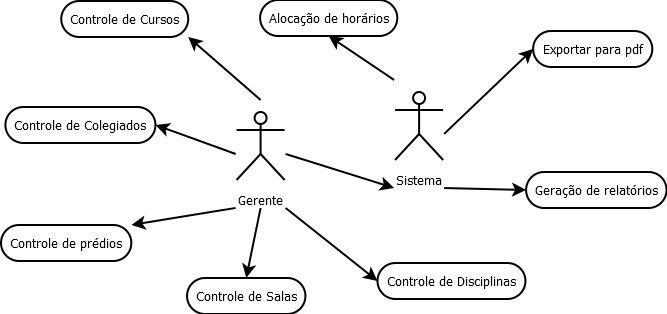
\includegraphics[scale=0.5]{diagramaCasoUso.png}
   		\\ \textbf{\footnotesize Fonte: Autor}
	\end{figure}


\subsubsecao{Diagrama de Atividade: Alocação}
	
	Descrever a rotina de atividades da alocação do sistema
	

\subsubsecao{Diagrama de Classe das controllers}
		
	Achar alguma referencia de diagrama de classe.

	Imagem do diagrama de classe das controllers

\subsubsecao{Diagrama de Classe das models}
	
	Imagem do diagrama de classe das models

\subsubsecao{Diagrama de Classe das views}
	
	Imagem do diagrama de classe das views

\subsubsecao{Modelagem de Dados}

	Achar alguma referencia de modelagem de dados

	Inserir imagem do modelo

		\begin{figure}[!htb]
   		\caption[Modelagem Banco de Dados]{Modelagem Banco de Dados}
   		\label{fig:figura3}
   		\centering
   		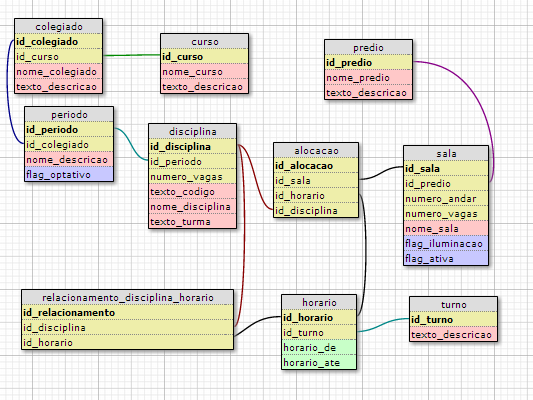
\includegraphics{modelagemBanco.png}
   		\\ \textbf{\footnotesize Fonte: Autor}
	\end{figure}

\subsecao{Interface}

	Achar alguma referencia sobre interface
	
	Twitter bootstrap.\par

\subsecao{Funcionalidades}

	O sistema consiste nas seguintes funcionalidades.

	1. Controle de cursos \par
	2. Controle de colegiados\par
	3. Controle de disciplinas\par
	4. Controle de salas\par
	5. Controle de prédios\par
	6. Alocação de horários\par
	7. Geração de relatórios\par
	8. Exportar para pdf\par



\subsecao{Dados de Entrada}

	Como serão inseriadas as informações, e quais são os dados de entrada

	Informados pelo gerente.

\subsecao{Alocação}

	Processa os dados de alocação

\subsecao{Relatórios}

	Geração dos relatorios determinados na analise do sistema, todos os relatorios podem ser exportados para pdf

\subsecao{Considerações Finais do Capítulo}

Considerações finais do capitulo

\capitulo{RESULTADOS E DISCUSSÕES}

\capitulo{CONCLUSÃO}

\iniciocapitulo
Discussão dos resultados obtidos na pesquisa, onde se verificam as observações pessoais do autor. Poderá também apresentar sugestões de novas linhas de estudo. A conclusão deve estar de acordo com os objetivos do trabalho. A conclusão não deve apresentar citações ou interpretações de outros autores.

\secao{Trabalhos futuros}

Criar um DW para geração dos relatorios de acordo com a dimensão escolhida.

Utilização de outros algoritimos para a resolução do problema ex. algoritimos evolutivos formiga entre outros.

\referencias{Referencias}

\capitulo{APÊNDICES}

\end{document}